\section{Additional Experimental Results} \label{section:supple:results}

The section presents complete experimental results and evaluations.
Please see the caption for the explanation of each figure.

%We here describe the details of the room annotation and object
%annotation experiments.


%Figure~\ref{fig:object_recog} shows the object annotation results, which
%turn out to be much more challenging than the room annotations, even
%with the state-of-the-art object
%detectors~\cite{berkeley_object_detection_software}.

% The scene recognition
% did not work well with the panorama images, and we render $400\times
% 300$ standard perspective images with the horizontal field of view of
% $90$ degrees. The results depend on the viewing directions and we
% experimented with the four algorithms as shown in
% Table~\ref{table:scene}.  The first algorithm, for example, picks the
% panorama closest to the room center, renders six uniformly overlapping
% images, and picks the scene type with the best average score. This
% performs the worst. The best algorithm looks at all the panorama images
% that are inside the room, but uses the single rendered image in which
% the room is the most visible in the top-down view. An observation is
% that poorly positioned panoramas tend to yield incorrect results but
% with very high confidence. A rather better strategy is to use the best
% viewing direction from the best panorama.

\clearpage
\begin{figure*}[!t]
%  \includegraphics[width=\textwidth]{../figures/closeups1.png}
 \includegraphics[width=\textwidth]{../figures/closeups1.pdf}
%		\includegraphics[width=\textwidth]{../figures/equal-sky.pdf}
%		\includegraphics[width=\textwidth]{../figures/salmon-palace.pdf}
	\caption{The figure shows that our offset-map reconstruction
 algorithm is able to produce highly regularized and compact 3D
 structure. We show three examples for each dataset.}
 \label{fig:detail0}
\end{figure*}

\clearpage
\begin{figure*}[!t]
% \includegraphics[width=\textwidth]{../figures/closeups2-2.png}
  \includegraphics[width=\textwidth]{../figures/closeups2.pdf}
 \caption{Continued.}  \label{fig:detail1}
\end{figure*}

\clearpage
\begin{figure*}
 \begin{center}
%  \includegraphics[width=\textwidth]{../figures/comp_meshes3.png}
    \includegraphics[width=\textwidth]{../figures/comp_meshes3.pdf}
 \end{center}
 \caption{Our structured model representation enables one to effectively
 hide (or add transparency to) back-facing surfaces such as ceilings and
 walls, at the level of structural elements as opposed to at the level of
 triangles. Meshes from existing algorithms only allow back-face culling per
 triangle and cause severe rendering artifacts for the aerial indoor
 scene visualization. }  \label{fig:comp_mesh0}
\end{figure*}

\clearpage
\begin{figure*}
 \begin{center}
%  \includegraphics[width=\textwidth]{../figures/comp_meshes4.png}
    \includegraphics[width=\textwidth]{../figures/comp_meshes4.pdf}
 \end{center}
 \caption{Continued.}  \label{fig:comp_mesh1}
\end{figure*}


\clearpage
\begin{figure*}
 \begin{center}
  \includegraphics[width=\textwidth]{../figures/show_texture.png}
%    \includegraphics[width=\textwidth]{../figures/show_texture.jpg}
%      \includegraphics[width=\textwidth]{../figures/show_texture.pdf}
 \end{center}
 \caption{The left and right shows our model with and without objects
 rendered.  Textures on the mesh models are computed for each piecewise
 planar surface by a combination of texture synthesis and inpainting
 techniques. Our structured representation essentially allows us to
 compute the texture for each structural element such as walls and
 floors, can effectively fill texture holes even behind objects.}
 \label{fig:texture0}
\end{figure*}

\clearpage
\begin{figure*}
 \begin{center}
  \includegraphics[width=\textwidth]{../figures/show_texture2.png}
%    \includegraphics[width=\textwidth]{../figures/show_texture2.pdf}
 \end{center}
 \caption{Continued.}  \label{fig:texture1}
\end{figure*}


\clearpage
\begin{figure*}[!t]
  \centering
%  \includegraphics[width=\textwidth]{../figures/room_recognition_stats0.png}
   \includegraphics[width=\textwidth]{../figures/room_recognition_stats00.pdf}
  \caption{Room annotations are obtained by using the state-of-the-art
 scene recognition system~\cite{mit_scene_demo_paper}. We experimented four
 different algorithms in choosing images to represent each room,
 yielding large performance variations. The annotation result for each
 room by each algorithm is shown in the table. We manually verified the
 results and highlight mistakes in red.}
 \label{fig:room_recog}
\end{figure*}

\clearpage
\begin{figure*}[!t]
  \centering
%  \includegraphics[width=\textwidth]{../figures/room_recognition_stats.png}
   \includegraphics[width=\textwidth]{../figures/room_recognition_stats_compressed.pdf}
  \caption{Continued.}
 \label{fig:room_recog1}
\end{figure*}

\clearpage
\begin{figure*}[!t]
  \centering
   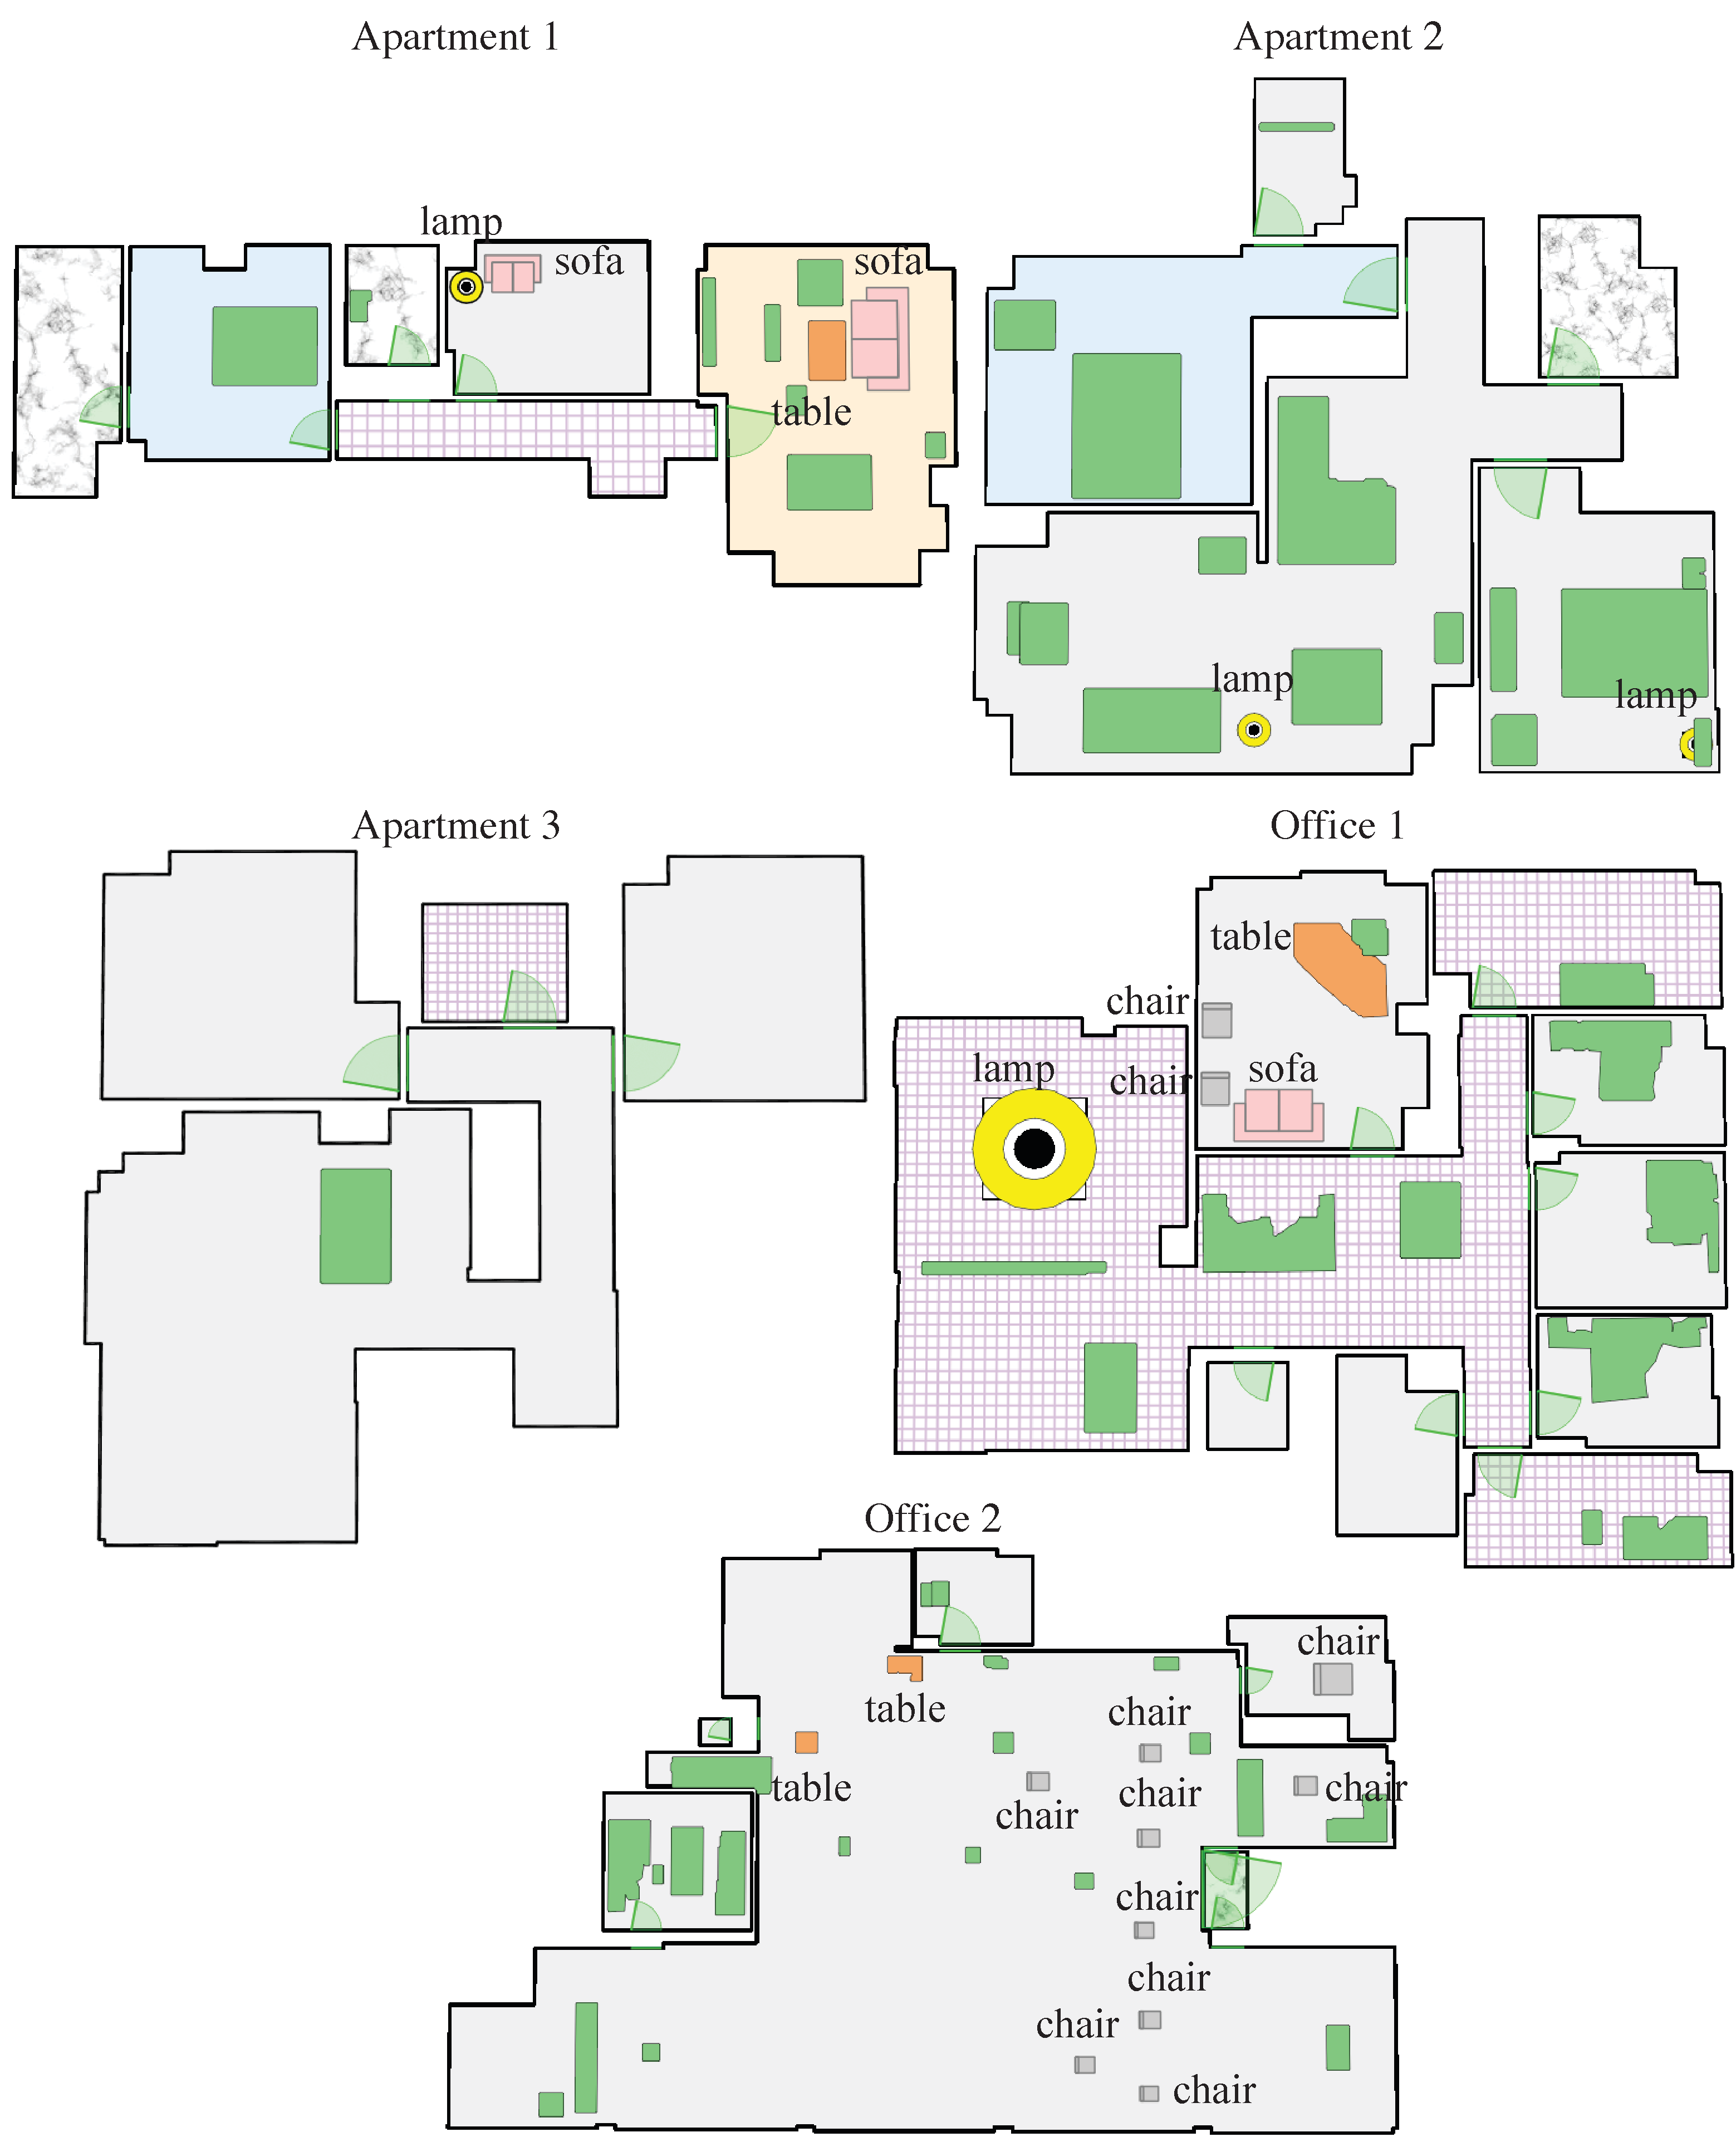
\includegraphics[width=\textwidth]{../figures/object_annotation.pdf}
  \caption{The object annotations turn out to be much more difficult
  than the room annotation. No texts are shown if an annotation cannot
  be associated. The segmentation results are good for major objects,
  and annotations, once obtained, are usually accurate.  However, most
  objects are missing annotations, especially in cluttered and small
  indoor rooms. A lot more improvements are to be made in this space.  }
  \label{fig:object_recog}
\end{figure*}

\clearpage
\begin{figure*}[!t]
  \centering
  \includegraphics[width=\textwidth]{../figures/object_reconstruction.png}
%   \includegraphics[width=\textwidth]{../figures/object_reconstruction.pdf}
  \caption{The figure illustrates our object reconstruction process for
  three rooms in our datasets.  From top to bottom: 1) a sample panorama
  image in the room; 2) the point-cloud in the room; 3) a point-cloud
  cluster for each object after removing points nearby the walls, the
  floors, or the ceilings; 4) point-cloud clusters after removing
  clusters that are too small or float in the air; and 5) the
 corresponding generated floorplan image in the room.
 % Object reconstruction pipeline. We want to reconstruction the
 %  objects in room shown in the first row. The second row shows all
 %  points inside the room. The third row shows the result after removing
 %  room structure(floors, ceilings and walls) and performing clustering
 %  to the remaining points. These segmentation results contain some
 %  floating objects(marked with green circles) and objects that are near
 %  room structure(marked with red circles), which can be replaced by room
 %  details. The fourth row shows the results after removing circled
 %  objects and small noisy objects, plus assigning colors from
 %  panoramas. The last rows shows the contours of objects from floorplan
 %view.}
 }
 \label{fig:objectreconstruction}
\end{figure*}

\clearpage
\begin{figure*}[!t]
  \centering
  \includegraphics[width=0.9\textwidth]{../figures/graphnew.pdf}
%   \includegraphics[width=0.9\textwidth]{../figures/graph_steps.png}
  \caption{Starting from the generation of the free-space end point
  evidence (left), we perform the room-segmentation and reconstruction
  (2-nd and 3-rd column).  More rooms are added and the room connection
  types are classified (4-th column). The white icon represents the
  ``door'', while the blue icon represents the ``merge'' classification.
  We finally get the structured graph representation as shown in the
  last column. Here we only show the spatial relationships for
  simplicity. }
\end{figure*}

\clearpage


